\documentclass[11pt,a4paper]{article}

\usepackage[utf8]{inputenc}
\usepackage[T1]{fontenc}
\usepackage[italian]{babel}
\usepackage{geometry}
\usepackage{graphicx}
\usepackage{booktabs}
\usepackage{array}
\usepackage{longtable}
\usepackage{enumitem}
\usepackage[hidelinks]{hyperref}
\usepackage{microtype}
\usepackage{xcolor}
\usepackage{fancyvrb}

\geometry{margin=2.4cm}
\setlist{nosep}

\title{Gestionale Affitti\\Relazione finale di Ingegneria del Software}
\author{Progetto individuale}
\date{Versione 1.0}


\begin{document}

\maketitle
\tableofcontents
\newpage

\section{Obiettivo e scope}

\emph{Gestionale Affitti} è un'applicazione web dimostrativa e mono-utente per la gestione essenziale di locazioni immobiliari ad uso abitativo. La versione 1.0 è volutamente limitata a due casi d'uso core, scelti per mantenere il progetto piccolo ma completo e tracciabile:

\begin{itemize}
  \item \textbf{UC-01 -- Registrare un contratto di locazione};
  \item \textbf{UC-02 -- Registrare il pagamento di un canone}.
\end{itemize}

L'unico attore diretto è il proprietario. L'inquilino è un concetto del dominio, ma non interagisce direttamente con il sistema. Restano fuori scope autenticazione, uso pubblico o multiutente, rinnovi operativi, pagamenti parziali, trasferimenti bancari reali, firma e registrazione fiscale del contratto.

La specifica completa e verificabile è mantenuta in \texttt{docs/requisiti.tex}. Durante la review finale è stato eliminato il precedente requisito prestazionale quantitativo di 1,5 secondi perché non era accompagnato da condizioni nominali e ambiente di misura riproducibili: è stato preferito rimuovere un requisito non realmente verificabile anziché introdurre un benchmark artificiale.

\section{Requisiti e casi d'uso}

UC-01 guida il proprietario attraverso cinque step: Immobile, Proprietario, Inquilino, Dati contrattuali e Riepilogo. I primi quattro step acquisiscono dati e aggiornano una bozza persistente; il riepilogo permette di tornare agli step completati, salvare la bozza, annullarla oppure confermare la registrazione definitiva.

UC-02 parte dalla selezione univoca dell'Immobile e dell'Inquilino, individua automaticamente la mensilità non pagata cronologicamente più vecchia fino al mese corrente e propone una preview. La conferma ricarica i dati persistiti, rivalida la competenza, ricalcola l'importo e registra il Pagamento usando la data corrente del server. La preview non è quindi una fonte autorevole.

\begin{figure}[p]
  \centering
  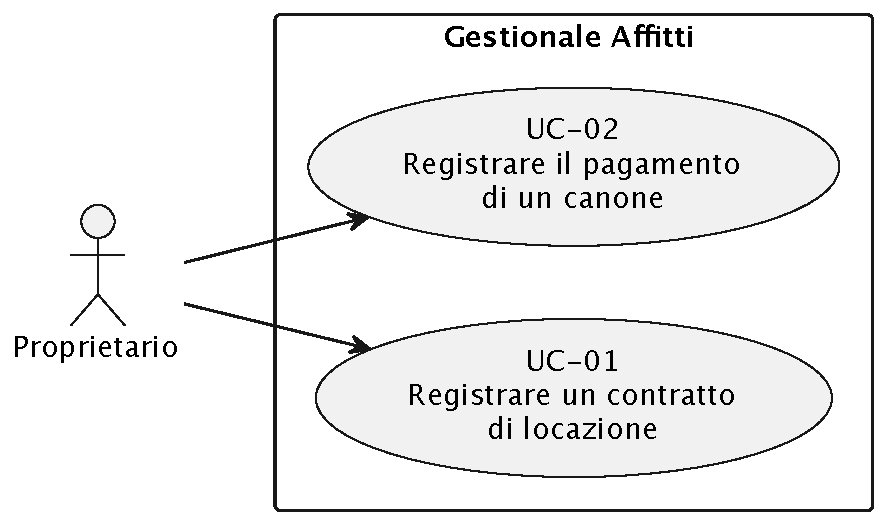
\includegraphics[
    width=0.96\textwidth,
    height=0.82\textheight,
    keepaspectratio
  ]{../uml/pdf/use-case.pdf}
  \caption{Use Case Diagram della versione 1.0}
\end{figure}
\clearpage

\section{Modellazione del dominio}

Il Domain Model mantiene separati i concetti stabili del dominio dai modelli temporanei del workflow applicativo. Le entità e value object principali sono \texttt{Persona}, \texttt{Immobile}, \texttt{Indirizzo}, \texttt{DatiCatastali}, \texttt{DocumentoRiconoscimento}, \texttt{Contratto}, \texttt{TipologiaContrattuale}, \texttt{Articolo} e \texttt{Pagamento}.

\texttt{BozzaContratto} non appartiene al Domain Model: rappresenta lo stato recuperabile della procedura di UC-01. Analogamente, \texttt{PagamentoDaRegistrare} è un application model usato per la preview di UC-02. La mensilità non è modellata come entità persistente, perché è derivabile dal periodo del Contratto, dai pagamenti registrati e dalla data corrente.

Le principali invarianti sono:

\begin{itemize}
  \item proprietario e inquilino devono essere Persone distinte;
  \item il giorno di pagamento è compreso tra 1 e 28;
  \item i periodi di Contratti dello stesso Immobile non possono sovrapporsi;
  \item per lo stesso Contratto può esistere al massimo un Pagamento per anno e mese di competenza;
  \item l'importo della prima e dell'ultima mensilità parziale è calcolato in pro-rata, con arrotondamento finale a due cifre decimali;
  \item la data corrente è una dipendenza autorevole del server e non un dato fornito dal client.
\end{itemize}

\begin{figure}[p]
  \centering
  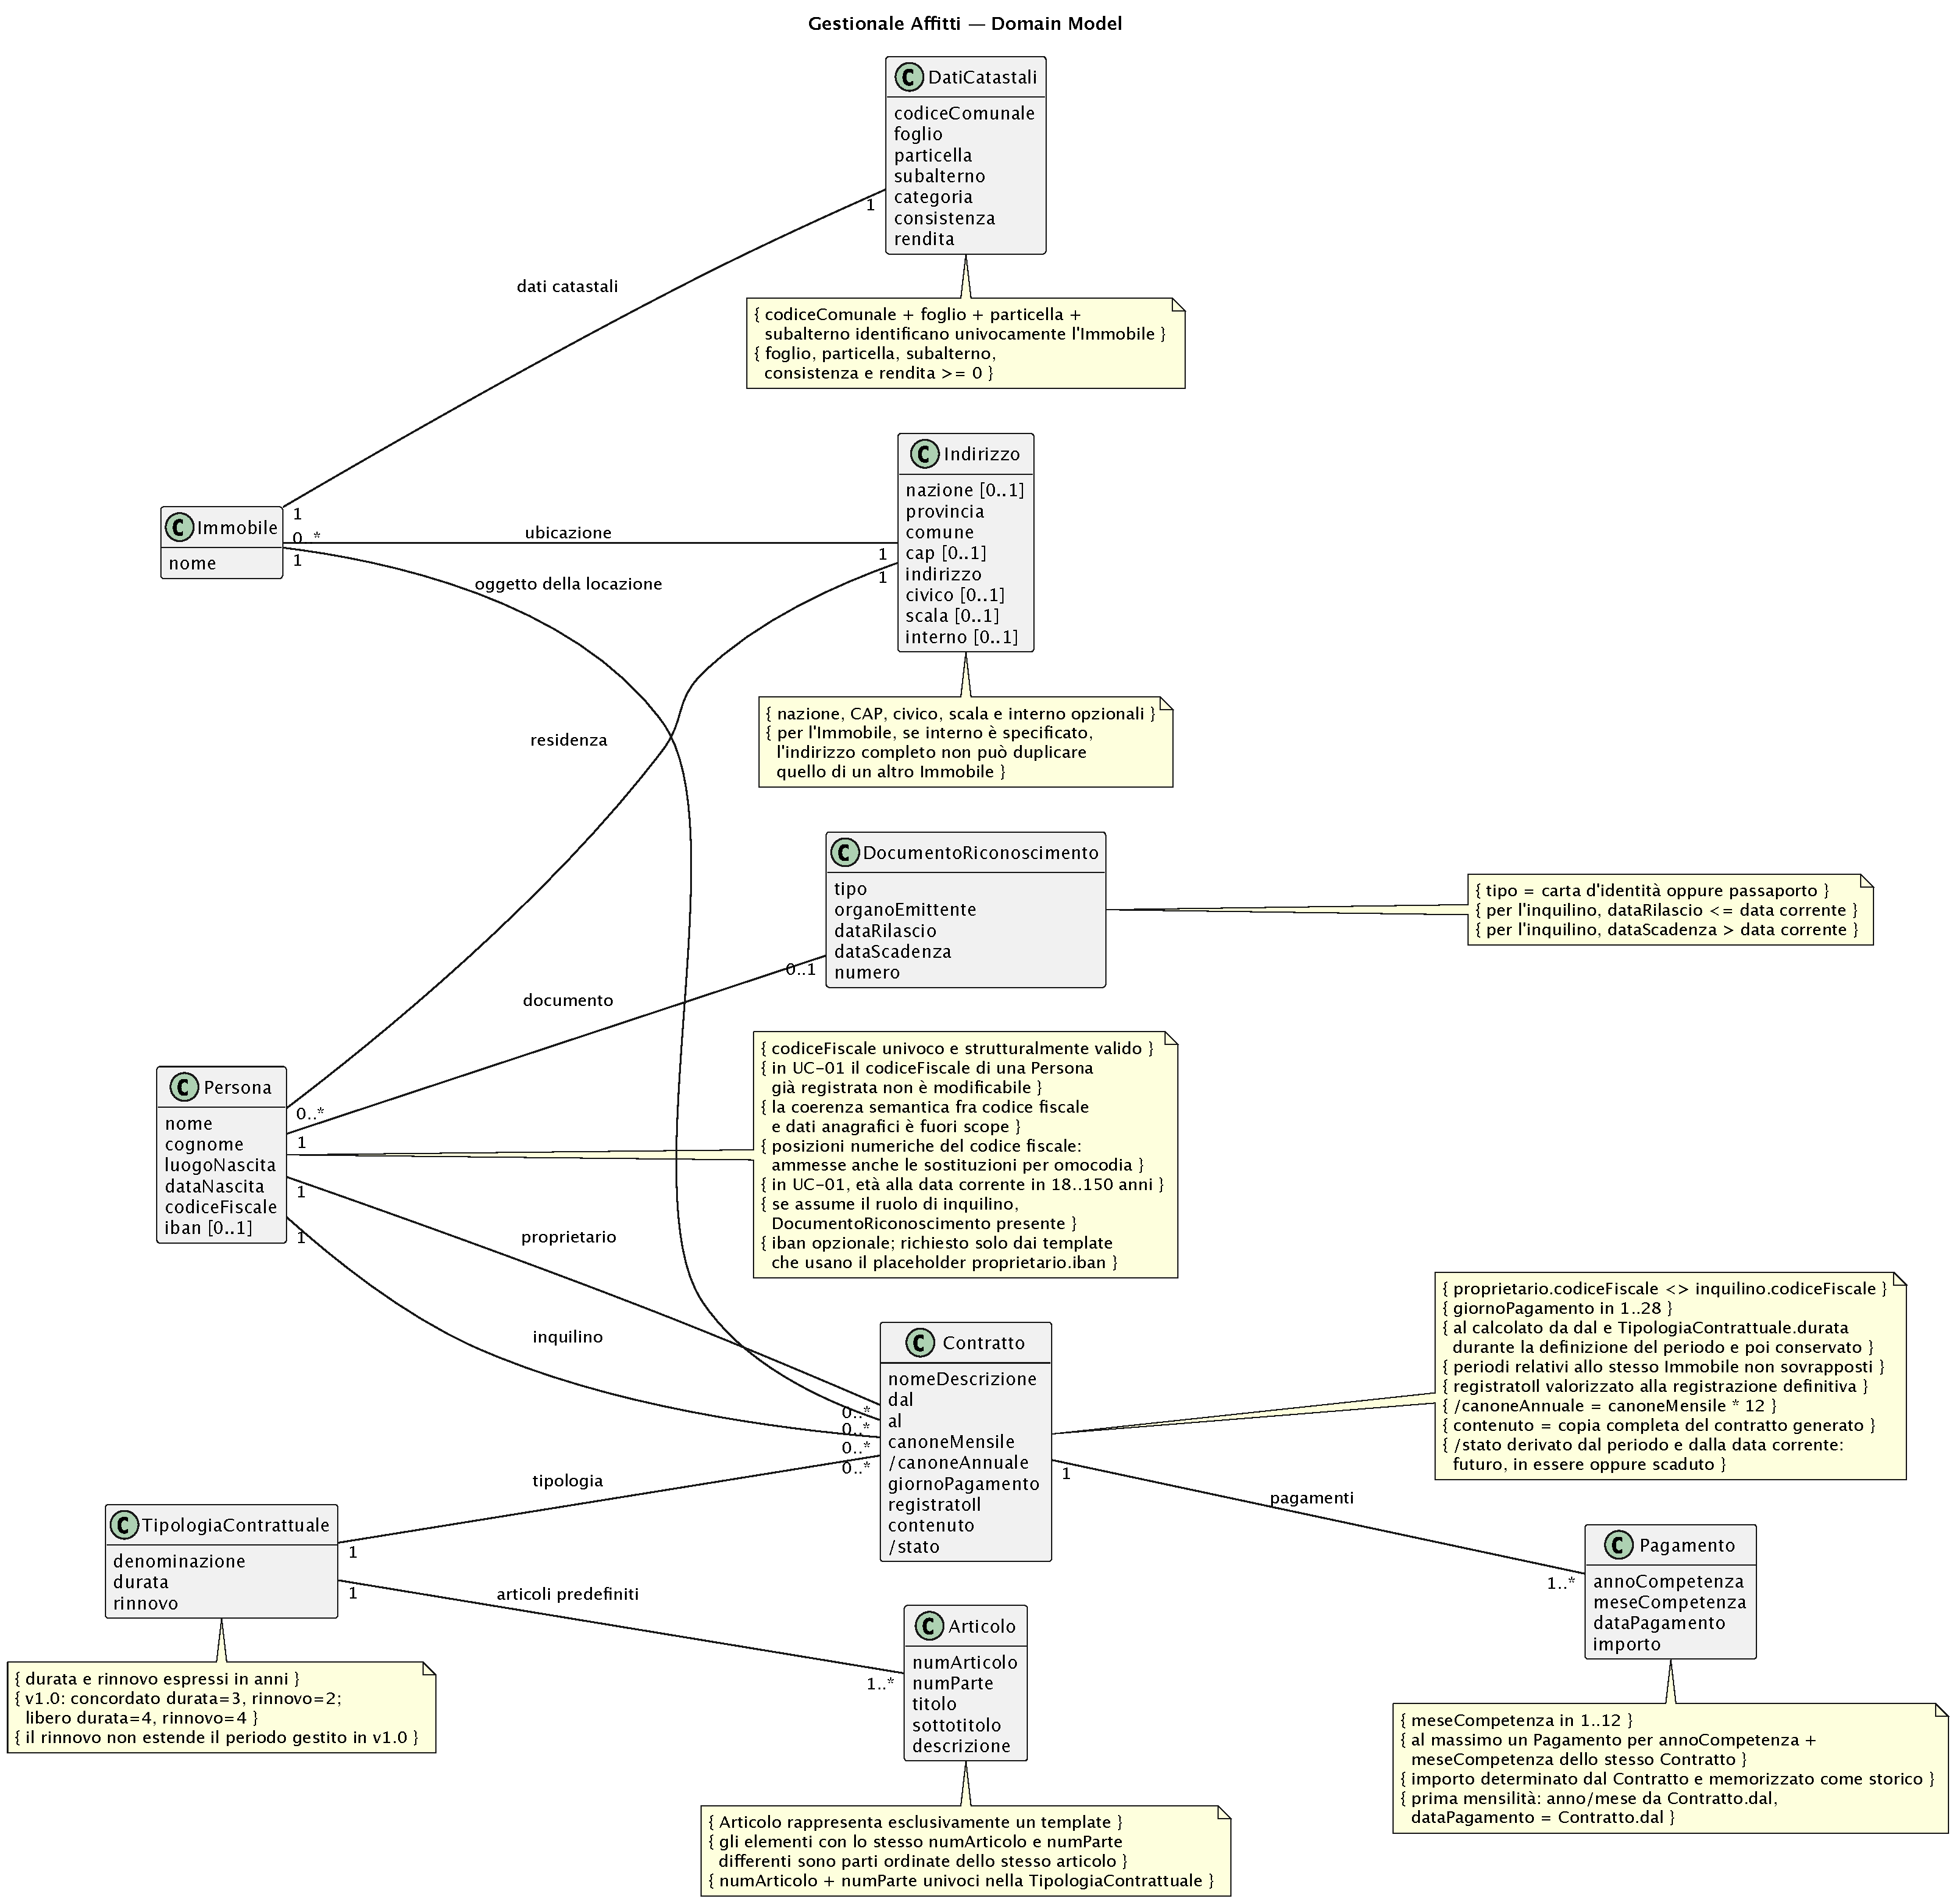
\includegraphics[
    width=0.96\textwidth,
    height=0.82\textheight,
    keepaspectratio
  ]{../uml/pdf/domain-model.pdf}
  \caption{Domain Model}
\end{figure}
\clearpage

\section{Architettura}

Il sistema adotta una struttura client-server e, all'interno del backend monolitico, una separazione layered. Le responsabilità logiche sono:

\begin{description}
  \item[web/interface] ricezione delle richieste HTTP, validazione formale, serializzazione e traduzione degli errori;
  \item[application] orchestrazione dei casi d'uso tramite \texttt{RegistraContrattoService} e \texttt{RegistraPagamentoService};
  \item[domain] regole stabili e invarianti del dominio;
  \item[infrastructure] PostgreSQL, mapping, transazioni, generazione HTML, data corrente e dettagli tecnici.
\end{description}

L'application layer dipende da porte definite sui bisogni dei casi d'uso. Le implementazioni concrete PostgreSQL dipendono da tali contratti. Il composition root in \texttt{src/web/compositionRoot.ts} è l'unico punto che conosce insieme i Service e le implementazioni infrastrutturali.

Per UC-01, \texttt{RegistrazioneContrattoPort} delimita l'operazione atomica di registrazione definitiva: dati definitivi collegati, Contratto e primo Pagamento vengono scritti nella stessa transazione PostgreSQL. Il cleanup della bozza è successivo al commit, così un suo eventuale fallimento non invalida un Contratto già registrato.

Per UC-02, \texttt{PagamentoRepository} è volutamente una porta di sola scrittura. I pagamenti storici vengono letti insieme al Contratto tramite \texttt{ContrattoRepository}; questa asimmetria evita due percorsi concorrenti per ricostruire lo stesso stato.

\begin{figure}[p]
  \centering
  \includegraphics[
    width=0.98\textwidth,
    height=0.82\textheight,
    keepaspectratio
  ]{../uml/pdf/class-diagram.pdf}
  \caption{Class Diagram di design}
\end{figure}
\clearpage

\section{SOLID e pattern}

\subsection{SRP}

Controller, Service, dominio e infrastruttura hanno motivi di cambiamento distinti. I Service non eseguono SQL né rendering concreto; i repository non contengono workflow; il dominio non dipende da Express o PostgreSQL.

\subsection{DIP}

Le dipendenze sostituibili sono invertite mediante porte: repository, generatore del documento e provider della data corrente. Questo permette di testare la business logic senza database o orologio reale.

\subsection{OCP}

Non vengono introdotte gerarchie preventive per le tipologie contrattuali, perché nella versione 1.0 differiscono per dati e template, non per famiglie di algoritmi. Il generatore del documento è invece isolato dietro una porta perché il formato di output rappresenta un punto di variazione concreto.

\subsection{Pattern non introdotti}

Strategy, Factory Method, Adapter e Observer sono stati valutati ma non adottati esplicitamente: nello scope corrente non risolvono un problema reale meglio della soluzione più semplice. Questa scelta evita overengineering e pattern dimostrativi non giustificati.

\section{UC-01: registrazione del contratto}

Il flusso di UC-01 utilizza bozze persistenti per consentire interruzione e ripresa. Nuovi Immobili, nuove Persone e modifiche alle Persone esistenti rimangono temporanei fino alla conferma. Il sistema valida codice fiscale, età, documento dell'Inquilino, eventuale IBAN richiesto dal template, durata del Contratto e sovrapposizione del periodo.

L'anteprima usa lo stesso generatore documentale della conferma, ma non produce scritture definitive. Alla conferma il Contratto viene ricostruito dalla bozza, i dati temporali vengono rivalidati, il documento viene rigenerato e conservato come contenuto storico. Viene inoltre creato il Pagamento della prima competenza.

\begin{figure}[p]
  \centering
  
\includegraphics[
    width=0.98\textwidth,
    height=0.82\textheight,
    keepaspectratio
  ]{../uml/pdf/sequence-uc01.pdf}
  \caption{Sequence Diagram di UC-01}
\end{figure}
\clearpage
\begin{figure}[p]
  \centering
  
\includegraphics[
    width=0.98\textwidth,
    height=0.82\textheight,
    keepaspectratio
  ]{../uml/pdf/activity-uc01.pdf}
  \caption{Activity Diagram di UC-01}
\end{figure}
\clearpage

\section{UC-02: registrazione del pagamento}

Il Service carica i Contratti della coppia Immobile--Inquilino, considera i Pagamenti già registrati e individua la prima competenza non pagata fino al mese corrente. Le mensilità future sono escluse; quella corrente è pagabile dal primo giorno anche se non è ancora dovuta.

Il Contratto calcola importo e scadenza. La preview espone anche lo stato dovuta/tardivo, ma alla conferma non viene considerata autorevole: il Service ricarica il Contratto, ricalcola la competenza più vecchia e rifiuta la conferma se la preview è diventata obsoleta. Il database mantiene inoltre un vincolo \texttt{UNIQUE (contratto\_id, anno\_competenza, mese\_competenza)} come protezione secondaria.

\begin{figure}[p]
  \centering
  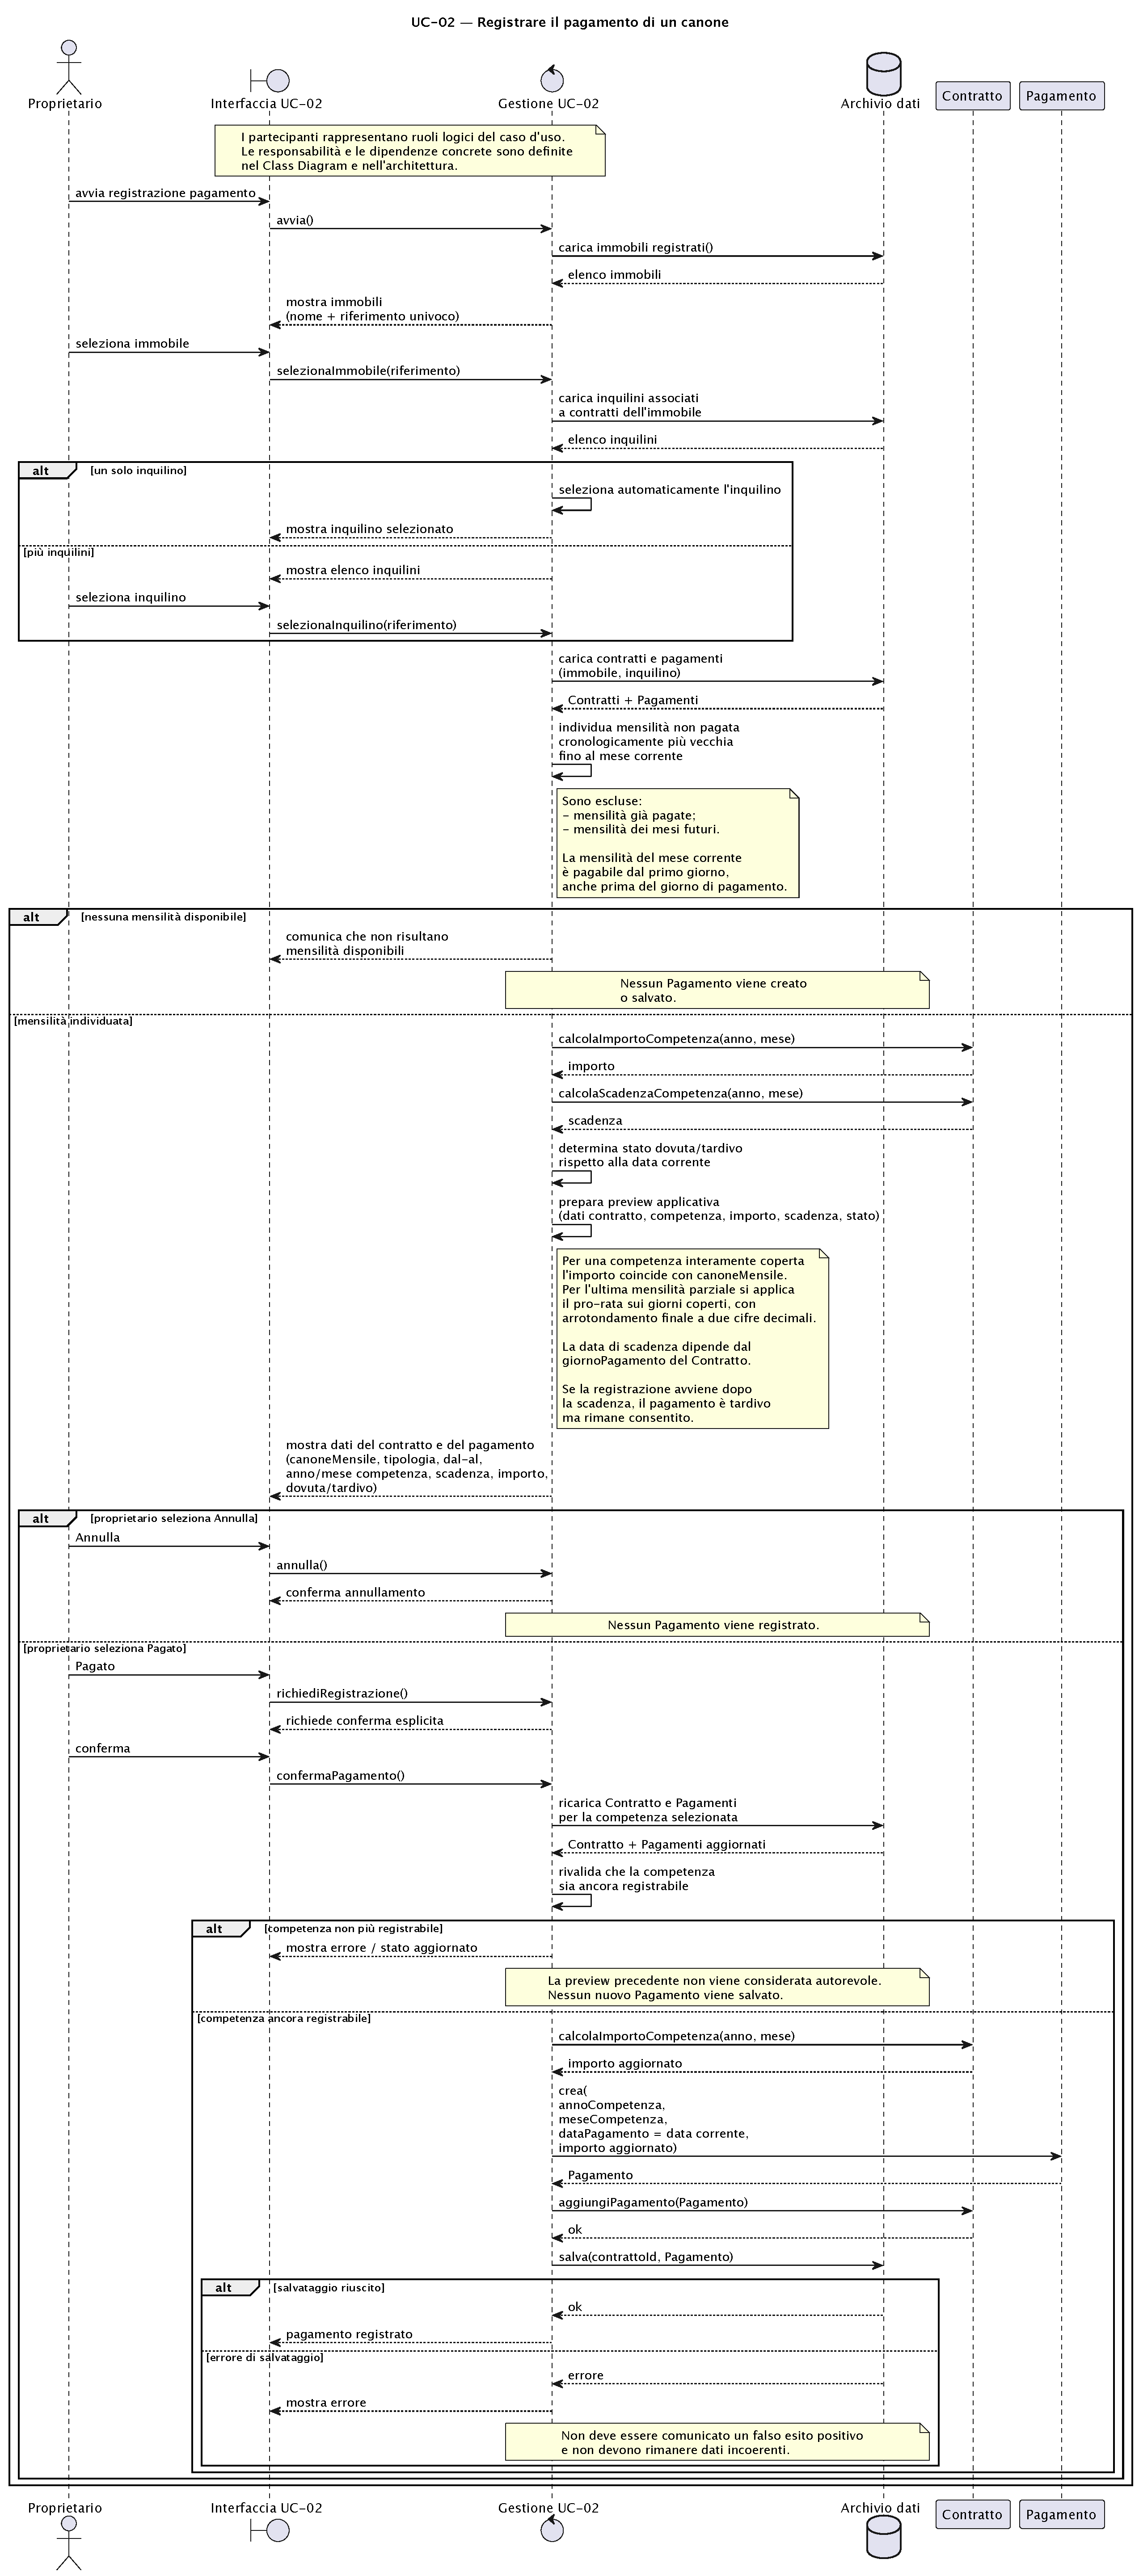
\includegraphics[
    width=0.98\textwidth,
    height=0.82\textheight,
    keepaspectratio
  ]{../uml/pdf/sequence-uc02.pdf}
  \caption{Sequence Diagram di UC-02}
\end{figure}
\clearpage

\section{Persistenza}

La persistenza usa PostgreSQL tramite il driver \texttt{pg} e SQL esplicito. Le migration sono versionate in \texttt{db/migrations/}; i template contrattuali iniziali sono JSON versionati in \texttt{db/seed/template/} e caricati con un seed idempotente e transazionale.

I dati definitivi sono relazionali. La bozza di UC-01 è l'unica struttura persistita come JSONB, perché rappresenta uno stato applicativo temporaneo ed eterogeneo. Il contenuto storico del Contratto è memorizzato come HTML in una colonna testuale e non viene rigenerato in seguito dai template correnti.

\section{Testing}

La strategia di test privilegia gli unit test sulle regole del dominio e sull'orchestrazione applicativa. Fake e stub sono usati per isolare repository e provider della data quando servono realmente; i test PostgreSQL sono riservati a query, mapping, vincoli e transazioni.

Le suite coprono:

\begin{itemize}
  \item regole di \texttt{Contratto}, \texttt{Persona}, \texttt{DocumentoRiconoscimento}, \texttt{DatiCatastali} e \texttt{Pagamento};
  \item lifecycle delle bozze e conferma di UC-01;
  \item generazione documentale e placeholder;
  \item repository e schema PostgreSQL;
  \item confine HTTP dei due casi d'uso;
  \item scenario end-to-end di UC-02 attraverso HTTP, application layer e PostgreSQL.
\end{itemize}

Lo scenario end-to-end di UC-02 verifica sia il flusso positivo sia un errore significativo: una preview diventa obsoleta prima della conferma e viene rifiutata senza creare duplicati o registrare una competenza differente.

\section{Quality gate e Continuous Integration}

Il comando canonico di verifica è:

\begin{Verbatim}[fontsize=\small]
npm run verify
\end{Verbatim}

Esso esegue build TypeScript, type-check dei test, ESLint e Jest. La pipeline GitHub Actions riproduce lo stesso quality gate in container, avvia PostgreSQL e usa \texttt{npm ci} per rispettare il lockfile. In questo modo la CI non introduce una definizione parallela di ``progetto valido'', ma automatizza il controllo già disponibile localmente.

\section{Tracciabilità}

La tracciabilità completa è mantenuta in \texttt{docs/tracciabilita.md}. Per entrambi i casi d'uso è possibile seguire il percorso:

\begin{center}
\textbf{Requisito $\rightarrow$ Acceptance Criteria $\rightarrow$ Caso d'uso $\rightarrow$ UML $\rightarrow$ Componente $\rightarrow$ Codice $\rightarrow$ Test}
\end{center}

Questa catena è usata anche come criterio di review: un componente importante deve essere giustificato da una responsabilità o da un requisito, e un requisito core deve avere evidenza implementativa e test significativa.

\section{Trade-off e limiti della versione 1.0}

Le principali scelte consapevoli sono:

\begin{itemize}
  \item monolite layered invece di servizi distribuiti, per evitare complessità non richiesta;
  \item SQL esplicito invece di ORM, perché lo scope rende gestibili query e mapping;
  \item nessun pattern GoF forzato;
  \item una porta \texttt{PagamentoRepository} orientata alla scrittura per evitare duplicazioni di lettura;
  \item nessun vincolo prestazionale quantitativo senza ambiente di misura riproducibile;
  \item contesto mono-utente, senza autenticazione e autorizzazione;
  \item gestione del solo periodo iniziale del Contratto, senza rinnovi operativi.
\end{itemize}

Questi limiti mantengono il progetto coerente con lo scope d'esame e rendono esplicito quali aspetti richiederebbero una revisione architetturale in un'evoluzione futura.

\section{Conclusioni}

La versione 1.0 implementa due casi d'uso completi e coerenti lungo l'intera catena di sviluppo: requisiti, modellazione, architettura, codice, test, CI e documentazione. La scelta progettuale dominante è mantenere responsabilità esplicite e dipendenze sostituibili senza introdurre complessità preventiva. Il risultato è un progetto contenuto, testabile e difendibile durante la discussione orale.

\end{document}
